\section{What fails for estimation, and what survives}
\label{sec:estimation}

We report the estimation outcome of the preregistered program exactly as the gate recorded it: the tuned soft-trim family fails as a deconfounding competitor, the failure is structural rather than a tuning artifact, and what survives is a dominance theorem for hard trimming together with a trim-then-regress recipe. The evaluation covered $97$ harmful cells ($16{,}520$ replications) of the simulator grid, with the preregistered no-regret requirement that the candidate's mean-bias norm lie within $1.05\times$ the best baseline in at least $95\%$ of harmful cells. The soft-trim family, comprising the EB-tuned spectral estimator, the linear special case of SDBoost \citep{nava2026sdboost}, and the default spectral deconfounding estimator of \citet{cevid2020spectral}, reaches no-regret in $4.12\%$ of harmful cells against the required $95\%$. A bias cut of at least $50\%$ relative to OLS holds in $40.21\%$ of cells against a required $70\%$, while the weaker $10\%$-cut condition holds in $82.5\%$: the family helps materially over doing nothing but never over hard-trim PCA. Winner counts are blunt: Onatski-selected hard trimming is the best baseline in $89$ of $97$ harmful cells, cross-validated ridge wins the other $8$, and the Bai--Ng selection rule \citep{bai2002determining}, the Cevid default, and the SDBoost-linear candidate never win a cell.

Two attribution checks, both predeclared, establish that the failure is structural. First, handing the family oracle knowledge of the variance-components tuning parameter raises no-regret only from $4.12\%$ to $6.2\%$: the ceiling of the family, not the quality of its tuning, is broken. Second, the SDBoost-linear candidate collapses identically to OLS, a phenomenon we now state as a lemma because it is an independent negative finding about a published method.

\begin{lemma}[SDBoost collapse]
\label{lem:sdboost-collapse}
Fix model M1 under A4a (dense $\beta$) with $c>1$ and bounded coordinate law $\sup_j z_j^2/d_j < \infty$ in probability, where $z_j = \sqrt{n}\,v_j'\hat\beta_{\mathrm{raw}}/\sqrt{d_j}$ are the $\sigma_y$-standardized spectral coordinates and $\hat\beta_{\mathrm{raw}} := V\,\mathrm{diag}(1/d)\,V'(X_c^\top Y_c/n)$ denotes the min-norm OLS coordinates in the sample eigenbasis $(V,d)$ of $X_c^\top X_c/n$. Let $(s_r^{2*}, s_e^{2*})$ denote the marginal maximum-likelihood variance components of the linear special case of \citet{nava2026sdboost}, and let $w_j = \bigl(1 + (s_r^{2*}/s_e^{2*})\, n\, d_j\bigr)^{-1}$ be the induced LAVA-type spectral weights (hybrid ridge-plus-sparse shrinkage in the style of \citealt{chernozhukov2017high}). All limits are in probability under the stated ledger. Then $(s_r^{2*}/s_e^{2*})\,n \to 0$ in probability and $\max_j |w_j - 1| \to 0$, whence for every boosting rate $\eta \in (0,1]$ and every $\varepsilon>0$ the boosting path satisfies $\|\alpha(m) - z/d\|_\infty \le \varepsilon\,\|z/d\|_\infty$ uniformly for all $m \ge m_0(\varepsilon,\eta)$: the path coincides with min-norm OLS along its entire tail, and any stopping rule that selects a late iterate returns exactly OLS with probability tending to one.
\end{lemma}

\begin{proof}[Proof sketch]
The profile log-likelihood is decreasing in the signal-variance component $s_r^2$ at almost every positive value under A4a: differentiating, stationarity would require a weighted average of $z_j^2/(s_e^2 + u\,d_j)$ (with $u = s_r^2 n$) to reach $1$, whereas each term converges to at most $1/(cu) < 1$, and the perpendicular block pushes the maximizer jointly toward larger $s_e^2$ and the corner $u=0$. The weights therefore tend to $1$ uniformly since $\sup_j d_j$ is tight, and $(1-\eta(1-\delta))^m \to 0$ geometrically gives the tail bound.
\end{proof}

The practical content of Lemma~\ref{lem:sdboost-collapse} is a silent failure mode: the EB tuning machinery runs, reports fitted variance components, and yet drives every spectral weight to $1$, so the published linear method inherits the full OLS bias while appearing to adjust. Our consolidated ledger records coefficient vectors equal to OLS to machine precision in $31$ of the $97$ harmful cells, with byte-identical mean-bias vectors in $42/97$ recorded in the earlier execution sweep. The scope guard matters: collapse requires the dense-signal coordinate bound, which fails under sparse or spike-aligned $\beta$, regimes where the variance components become identifiable and the method does useful work; the lemma indicts it precisely where its deconfounding claim was aimed.

The dominance side is captured by a theorem for spectral-weight estimators. Define $\mathcal{W}_+$ as all estimators of the form $\hat\beta_m = V\,\mathrm{diag}(m_j(\hat d))\,V'\,b_{\mathrm{raw}}$ with $b_{\mathrm{raw}} = X_c'Y_c/n$ and weights $m_j \ge 0$ that are measurable functions of the sample spectrum alone. Min-norm OLS ($m_j = 1/d_j$), ridge, hard trims, soft trims, lava-shaped weights, and the SDBoost path are all members. Two tempting generalizations are excluded deliberately. Sign-flipping tricks, which reverse coordinate signs according to their estimated response linkage, exit the class because they use information beyond the spectral coordinates and destroy the nonnegativity that the transmission bookkeeping requires. Projection-type maps written as $V\operatorname{diag}(w)V'$ without the $1/d_j$ division are excluded because they are not estimators of $\beta$: they transmit confounding at $O(\sqrt{l})$ strength instead of the cap law $O(\sqrt{l}/(1+l))$, a pitfall our first falsifier run caught and archived.

Two functionals organize the bookkeeping, both read loading- and beta-conditionally as in Section~\ref{sec:capture}. The confounding-attributed \emph{transmission} of a member $m$ on spike direction $q_j$ is its twin difference
\[
\Delta_j(m):=\E[\langle\hat\beta_m,q_j\rangle\mid\gamma]-\E[\langle\hat\beta_m,q_j\rangle\mid\gamma=0],
\]
and its \emph{fidelity} $\phi_j(m)$ is defined through the null arm,
\[
B_{0,j}(m):=\E[\langle\hat\beta_m-\beta,q_j\rangle\mid\gamma=0],
\qquad
\phi_j(m):=1+\frac{B_{0,j}(m)}{\langle\beta,q_j\rangle},
\]
so fidelity records how much of the structural component survives on that coordinate ($\phi_j=0$ exactly when the member discards the direction entirely). On every fixed direction $j$, subcritical or not, the transmission law is $\Delta_j(m)=T_j(m)\,a_j\,\gamma_j$ with $a_j=\sqrt{l_j}/(1+l_j)$ and $T_j(m)$ the resolvent-channel capture inherited from Section~\ref{sec:capture} ($T_j=\mathrm{cap}_j$ for min-norm OLS, $\mathrm{cap}_j(\lambda)$ for ridge, indicator-valued for hard trims), while the fit-artifact channel is $B_{0,j}=-(1-\phi_j)\langle\beta,q_j\rangle$.

\begin{theorem}[Hard-trim transmission dominance on subcritical cells]
\label{thm:hardtrim}
Fix a grid cell in which every factor spike is subcritical (so no direction detaches from the bulk edge) and A4a holds. Work at deterministic-equivalent level, conditionally on the loadings and $\beta$. All claims are deterministic-equivalent statements with remainders $o(1)$ conditionally on loadings and $\beta$; no distributional limit is asserted. Then: (i) within $\mathcal{W}_+$ minus the zero estimator, the minimal attainable confounding-attributed directional bias is zero, attained exactly by members whose fidelity $\phi_j$ vanishes on every subcritical direction, in particular hard trims whose retained set excludes those directions; (ii) any member with $\phi_j \ge \varepsilon_j > 0$ on some subcritical direction $j$ incurs directional confounding transmission $\Delta_j \ge \varepsilon_j\, a_j |\gamma_j| - o(1)$ with $a_j = \sqrt{l_j}/(1+l_j)$, a strict loss at every link strength bounded away from zero, however tuned; and (iii) on a fully subcritical spectrum no coordinate ratio statistic crosses the Onatski critical value, so their edge-delimited rule \citep{onatski2010determining} returns $k=0$ with probability tending to one (the rule is designed for spiked alternatives; under a pure bulk every candidate edge falls below threshold). For the vector target this makes explicit that no nontrivial member of $\mathcal{W}_+$ attains zero total bias without discarding every direction, which is precisely why vector estimation is declared unrecoverable in this regime; for the scalar treatment target, however, the corresponding trim arm reduces to univariate adjustment of $D$, which transmits no design-borne confounding while keeping the treatment identified, and this asymmetry is what Section~\ref{sec:benchmarks} exploits.
\end{theorem}

All three statements above concern the confounding-attributed transmission functional; total mean-bias norm additionally contains the fidelity-loss artifact $B_{0,j}$, which trims pay on discarded signal directions.

\begin{proof}[Proof sketch]
On a subcritical direction there is no BBP enhancement to separate the two arms, so both are governed by one coordinate multiplier: writing $\rho_j(m)$ for the realized multiplier on $\langle\beta,q_j\rangle$ in the null arm, $\E[\langle\hat\beta_m,q_j\rangle\mid\gamma=0]=\rho_j(m)\,\langle\beta,q_j\rangle+o(1)$ (so fidelity is definitional: $\phi_j=\rho_j$), the Section~3 ledger gives $B_{0,j}=-(1-\phi_j)\langle\beta,q_j\rangle$ as stated; below the BBP threshold no capture-enhancement channel operates, so the twin arm shares the same multiplier, $T_j=\rho_j$, and hence $\Delta_j\ge0$ with equality iff $\rho_j=0$, proving (i) together with the ``attained exactly by'' clause; and (ii) follows because $\phi_j\ge\varepsilon_j$ forces $T_j=\phi_j\ge\varepsilon_j$, so $\Delta_j\ge\varepsilon_j a_j|\gamma_j|$. For (iii), on a fully subcritical spectrum the Onatski edge rule returns $k=0$ consistently, so the trim realizes the zero-fidelity member.
\end{proof}

\begin{corollary}[Why soft tuning must lose]
\label{cor:kill}
Every soft family in the roster places strictly positive weight on subcritical directions by construction (at deterministic-equivalent level ridge keeps weight of order $d_j/(d_j+\lambda)$ on subcritical directions for fixed $\lambda$, and EB weights collapse toward $1$ by Lemma~\ref{lem:sdboost-collapse}), so no amount of tuning removes the transmission that the weight shape itself forces. Under A4a the fidelity-loss artifact is small per direction ($|\langle\beta,q_j\rangle|=O_p(p^{-1/2})$), so total-bias comparisons in harmful cells are governed by the transmission term just characterized. The frozen attributions are therefore consistent with the theorem but remain empirical verdicts rather than corollaries: the oracle-tau ceiling of $6.2\%$, Onatski as best baseline in $89$ of $97$ harmful cells, and byte-equality of SDBoost with OLS on the collapsed cells.
\end{corollary}

Honesty about scope: Theorem~\ref{thm:hardtrim} is closed at deterministic-equivalent level for the subcritical claim, which is exactly the harmful-and-invisible region; the mixed and supercritical cells, where retained-direction fidelities bind and soft weights trade transmission against shrinkage along a Pareto curve, are recorded descriptively through the crossover strip rather than theorized. Finite-sample refinements (the BGN overlap factor on retained directions) are verified numerically, and the transmission law reproduces the measured confounding functional in frozen anchor cells to within $0.2\%$ and $2.5\%$.

What survives is substantial. First, trim-then-regress: in the M2 weak-treatment block (sparse treatment projection, $\|\delta\|=0.3$, known $\tau_{\mathrm{true}}$), mean absolute $\tau$ errors for the Onatski-trimmed estimator stay flat across the aspect range ($0.047$, $0.035$, $0.042$ at $c = 0.2, 0.8, 2.0$) while naive OLS inflates roughly six-fold across $c=0.2,0.8,2.0$ (frozen magnitudes $0.064$, $0.058$, $0.391$; the middle cell sits at the crossover trough before the $c>1$ attenuation switches on, the fresh-run signed mean at the last cell is $-0.403$, reconciled in Section~\ref{sec:capture}), and Onatski rank selection matches the oracle-$r$ trim exactly in every cell; Section~\ref{sec:benchmarks} replicates the pattern on real econometric geometry ($\tau$ error $0.173$ trimmed versus $0.421$ for OLS). Second, the characterization itself is robust: across $28$ variant arms covering $t$-distributed errors, Rademacher-half loadings, row-heteroskedastic noise, correlated factors, $r \pm 1$ misspecification, and sparse confounding, the median ratio of the EB-tuned bias norm to the best baseline ranges only from $1.48$ ($r$ misspecification, least damaging) through $2.26$ (Gaussian reference) to $5.26$ (heteroskedasticity, where soft weights misread the inflated bulk), and no variant ever flips a winner, so the qualitative phase-diagram structure of Figure~\ref{fig:phasediagram} survives every perturbation. One diagnostic sub-rule could not be evaluated on variant arms because detection statistics were stored on the main arm only; this scope cut is flagged in the gate-checks output rather than silently dropped. Computationally, the full estimator roster runs in $0.02$\,s at $(n,p)=(1000,1000)$, $1.53$\,s at $(4000,8000)$, and $0.16$\,s at $(8000,1600)$ per replication, scaling with $\min(n,p)^2$ to $\min(n,p)^3$ inside the memory ceilings throughout.

Figures~\ref{fig:crossover} and~\ref{fig:phasediagram} summarize the landscape: the crossover strip shows the near-oracle mean-bias floor of approximately $0.08$ that Onatski truncation maintains across the entire link-strength grid, below every soft competitor everywhere, while the empirical phase diagram marks the subcritical region where Theorem~\ref{thm:hardtrim} applies and the mixed region where the families nearly tie.

\begin{figure}[t]
\centering
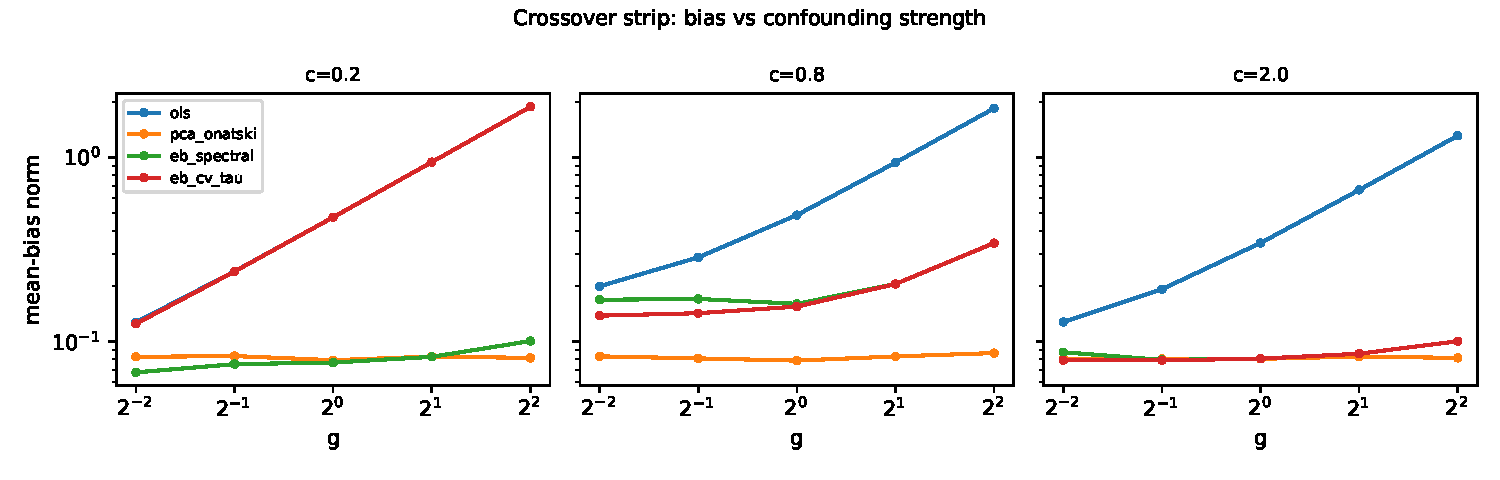
\includegraphics[width=\linewidth]{figures/crossover_curves.pdf}
\caption{Mean-bias norms against link strength $g$ for the soft-trim family and the leading baselines. Onatski-selected hard trimming maintains a near-oracle floor across the grid; smoothly down-weighted competitors cannot reach it, and the SDBoost-linear path sits on top of OLS on collapsed cells.}
\label{fig:crossover}
\end{figure}

\begin{figure}[t]
\centering
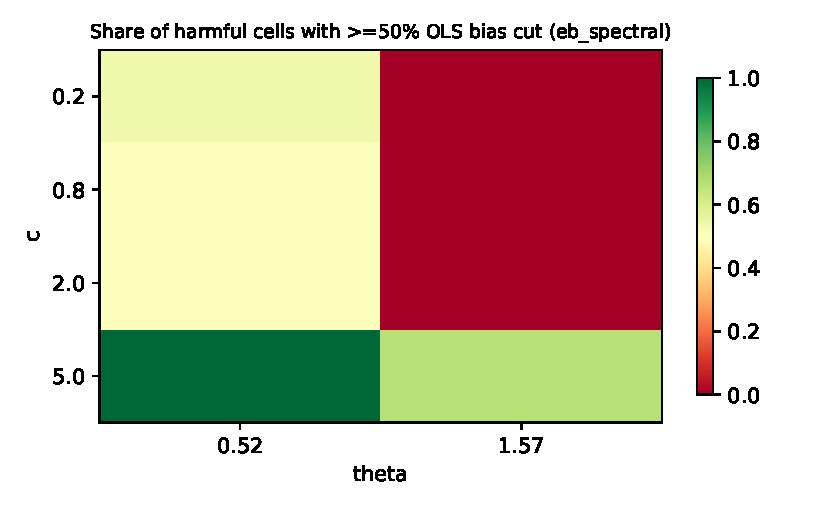
\includegraphics[width=\linewidth]{figures/bias_phase_diagram_empirical.pdf}
\caption{Empirical bias phase diagram over $(c, g)$: the subcritical region where Theorem~\ref{thm:hardtrim} forces the dominance of hard trimming, the supercritical region where confounding becomes visible and estimable, and the mixed boundary traced by the crossover measurements.}
\label{fig:phasediagram}
\end{figure}
